\chapter{2020}
\section*{一、选择题(本大题共 15 小题,每小题 2 分,共 30 分)}

1. 设三个函数 \(\mathrm{f},\mathrm{g},\mathrm{h}\) 分别为 \(\mathrm{f}\left( \mathrm{n}\right)  = {1000}{\mathrm{n}}^{3} + {\mathrm{n}}^{2} + {1000},\mathrm{\;g}\left( \mathrm{n}\right)  =\)  \({1000}{n}^{3} + {5000}{n}^{2},h\left( n\right)  = {n}^{3/2} + {5000}{nl}{gn}\) ,下列哪个关系不成立 (\_\_\_\_\_)。

A. \(\mathrm{f}\left( \mathrm{n}\right)  = \mathrm{O}\left( {\mathrm{g}\left( \mathrm{n}\right) }\right)\) B. \(\mathrm{g}\left( \mathrm{n}\right)  = \mathrm{O}\left( {\mathrm{f}\left( \mathrm{n}\right) }\right)\)

C. \(\mathrm{h}\left( \mathrm{n}\right)  = \mathrm{O}\left( {\mathrm{n}}^{3/2}\right)\) D. \(\mathrm{h}\left( \mathrm{n}\right)  = \mathrm{O}\left( {\mathrm{{nl}}\mathrm{{gn}}}\right)\)

2. 已知 \(\mathrm{P}\) 结点是某双向链表的一个结点,在 \(\mathrm{P}\) 结点后插入一个新结点 \(\mathrm{S}\) 的语句序列是(\_\_\_\_\_)。

A. S->prior=P->prior;
P->prior=S;
S->next=P;
P->prior->next=S;

B.
S->prior=P;
S->next=P->next;
P->next->prior=S;
P->next=S;

C.
S->prior=P->prior;
P->prior->next=S;
P->prior=S;
S->next-=P;

D.
S->prior=P;
S->next=P->next;
P->next=S;
P->next->prior=S;

3. 栈在(\_\_\_\_\_)中应用。

A. 递归调用 B. 子程序调用

C. 表达式求值 D. A, B, C

4. 若用一个大小为 6 的数组来实现循环队列, 且当前 rear 和 front 的值分别为 0 和 3 , 当从队列中删除一个元素, 再加入两个元素后, rear 和 front 的值分别为(\_\_\_\_\_)。

A. 1 和 5 B. 2 和 4 C. 4 和 2 D. 5 和 1

5. 设完全二叉树的第 \(\mathrm{i} = 6\) 层有 24 个叶结点,则此树最多有 (\_\_\_\_\_)个结点。( \(i \geq  1\) )

A. 55 B. 79 C. 81 D. 127

6. 下列序列(\_\_\_\_\_)不是堆？

A.12,35,39,57,86,48,42,73,66,100

B.12,70,33,65,24,56,48,92,86,33

C.06,12,20,30,52,23,42,38,103,97,66,56

D.05,23,20,35,28,38,29,61,56,76,40,100

7. 将下图中二叉树按中序线索化,结点 \(\mathrm{f}\) 的右指针和结点 \(\mathrm{g}\) 的左指针分别指向结点 (\_\_\_\_\_)。

\begin{center}
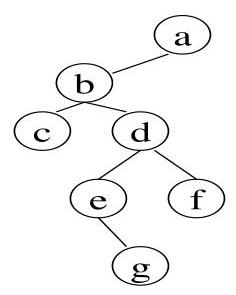
\includegraphics[width=0.2\textwidth]{images/2020/choice_7.jpg}
\end{center}
\hspace*{3em} 

A. d, e B. b, d

C. \(\mathrm{d},\mathrm{b}\) D. \(\mathrm{a},\mathrm{e}\)

8. 在 Huffman 编码中, 若编码长度只允许小于等于 5 , 则除了已对两个字符编码为 0 和 10 外,还可以最多对(\_\_\_\_\_) 个字符编码。

A. 5 B. 6 C. 7 D. 8

9. 设 \(\mathrm{G}\) 是一个非连通无向图,有 28 条边,则该图的顶点数至少有(\_\_\_\_\_)个。

A. 7 B. 8 C. 9 D. 10

10. 对于一个有向图,若一个顶点的度为 \(\mathrm{k}1\) ,出度为 \(\mathrm{k}2\) ,则对应逆邻接表中该顶点的入边表中的边结点数为(\_\_\_\_\_)。

A. k1 B. k2 C. k1-k2 D. \(\mathrm{k}1 + \mathrm{k}2\)

11. 在下图中所示的 AOE (Activity On Edge) 网中, 关键路径长度为(\_\_\_\_\_)。

A. 23 B. 22 C. 16 D. 13

\begin{center}
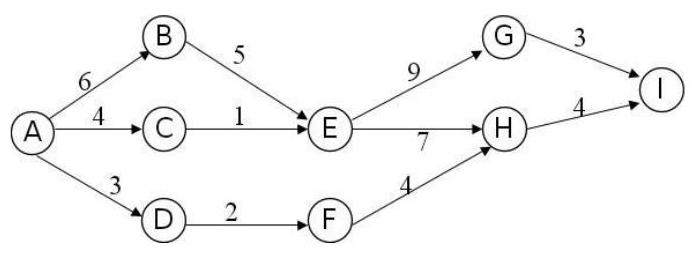
\includegraphics[width=0.5\textwidth]{images/2020/choice_11.jpg}
\end{center}
\hspace*{3em} 

12. 如果一个有向图具有拓扑有序序列, 并且顶点按拓扑有序序列编号,那么其邻接矩阵必定为(\_\_\_\_\_)。

A. 对称矩阵 B. 三对角矩阵

C.上三角矩阵 D. 下三角矩阵

13. 已知一个长度为 18 的有序顺序表中, 若采用折半查找法查找第 12 个元素,则比较次数是(\_\_\_\_\_)。

A. 3 B. 4 C. 5 D. 6

14. 如果将学校所有同学按照生日(不考虑年份,只考虑月、日) 来排序,那么下列排序算法中排序速度最快的算法是 (\_\_\_\_\_)。

A. 归并排序 B. 希尔排序

C. 快速排序 D. 基数排序

15. 下列(\_\_\_\_\_)不是 AVL 树(平衡二叉树)。

A
\begin{center}
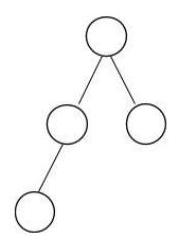
\includegraphics[width=0.2\textwidth]{images/2020/choice_15_A.jpg}
\end{center}
B
\begin{center}
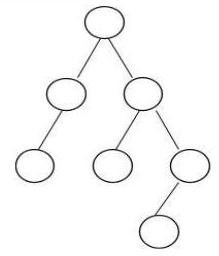
\includegraphics[width=0.2\textwidth]{images/2020/choice_15_B.jpg}
\end{center}
C
\begin{center}
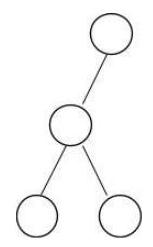
\includegraphics[width=0.2\textwidth]{images/2020/choice_15_C.jpg}
\end{center}
D
\begin{center}
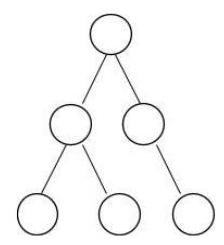
\includegraphics[width=0.2\textwidth]{images/2020/choice_15_D.jpg}
\end{center}

\section*{二、填空题 (本大题共 15 小题, 每小题 2 分, 共 30 分)}

1. 考虑函数 \(f\left( n\right)  = n\log n\) 和 \(g\left( n\right)  = {n}^{a}\) ,其中 \(a\) 是实数。在下列空白处填写合适的数学符号(比如 \(> , \geq  , < , \leq\) 等),使得下列函数关系成立。 \(\mathrm{f} = \mathrm{O}\left( \mathrm{g}\right)\) :当 \(\mathrm{a}\) \_\_\_\_\_1； \(\mathrm{g} = \mathrm{O}\left( \mathrm{f}\right)\) :当 \(\mathrm{a}\) \_\_\_\_\_1。

2. 表达式 a*b-c-d\$e\$f-g-h*i 中,运算符的优先级由高到低依次为 \(- , * ,\$\) ,且均右结合,则相应的后缀式是\_\_\_\_\_。

3.7 个元素 \(\mathrm{a}\) 、 \(\mathrm{b}\) 、 \(\mathrm{c}\) 、 \(\mathrm{d}\) 、 \(\mathrm{e}\) 、 \(\mathrm{f}\) 和 \(\mathrm{g}\) 顺序入栈。在栈上做了 5 次弹出操作,每个出栈的元素被插入到一个队列中。从队列中删除 3 个元素并将其推回到栈中。现在, 从栈中弹出一个元素, 弹出的这个元素是\_\_\_\_\_。

4. 设一个稀疏矩阵有 1000 行 850 列, 其中有 1000 个非 0 数据元素。设每个整数值占 \(2\mathrm{\;B}\) ,数据元素值占 \(4\mathrm{\;B}\) ,则用三元组表存储该矩阵时所需字节数是\_\_\_\_\_。

5. 一棵二叉排序树 (BST, binary search/sort tree) 的后序遍历序列是15,10,23,25,20,35,42,39,30。请给出这棵树的前序遍历序列:\_\_\_\_\_。

6. 如果 T1 是由有序树 \(\mathrm{T}\) 转换成的二叉树,那么 \(\mathrm{T}\) 中结点的后根遍历顺序对应 T1 中结点的\_\_\_\_\_ 遍历。

7. 设一棵树中只有度为 0 和度为 3 的结点,则该树的第 \(\mathrm{i}\) 层 \(\left( {i \geq  1}\right)\) 的结点个数最多为\_\_\_\_\_。

8. 在一个图中, 所有顶点的度数之和等于图的边数的\_\_\_\_\_倍。

9. 一个有向图的邻接表存储如下图所示, 现按深度优先搜索方式从顶点 \(\mathrm{F}\) 出发执行一次遍历,则得到的顶点系列是\_\_\_\_\_。

\begin{center}
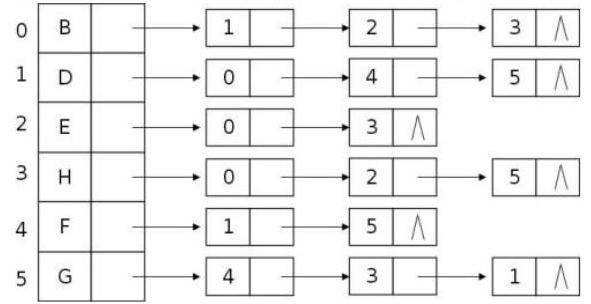
\includegraphics[width=0.5\textwidth]{images/2020/blank_9.jpg}
\end{center}
\hspace*{3em} 

10. 设一个 \(\mathrm{n}\) 个顶点的带权连通图有 \({\mathrm{n}}^{1/2}\log \mathrm{n}\) 条边,则应该选用\_\_\_\_\_(从 Prim, Kruskal 中选择一个填空)算法求这个图的最小生成树, 从而使计算时间较少。

11. 对于长度为 9 的有序顺序表, 若采用折半查找, 在相等查找概率情况下查找成功的平均查找长度为\_\_\_\_\_,查找不成功的平均查找长度为\_\_\_\_\_。

12. 将 10 个元素散列到大小可容 100000 个元素的散列表中,\_\_\_\_\_产生冲突。(请在“一定会”、“一定不会”、“仍然可能会”这些术语中选择正确的进行填空)

13. 数组 \(A\) 中,每个元素 \(A\) 的长度为 3 个字节,行下标 \(i\) 从 1 到 8, 列下标 \(j\) 从 1 到 10,从首地址 1000 开始连续存放在存储器内, 该数组按行优先存放时,元素 \(A\left\lbrack  8\right\rbrack  \left\lbrack  5\right\rbrack\) 的起始地址为\_\_\_\_\_。

\vspace{14em}

14. 如果有一个时间复杂度为 \(\mathrm{O}\left( {\mathrm{n}}^{2}\right)\) 的算法(比如冒泡排序、选择排序或插入排序等),在有 200 个元素的数组上运行需要耗时 3.2 毫秒。那么, 在类似的有 40000 个元素的数组上运行, 需要\_\_\_\_\_秒时间。

15. 顺序文件中,要存取第 i 个记录,必须先存取\_\_\_\_\_个记录。

\section*{三、综合应用题 (本大题共 6 小题, 每小题 10 分, 共 60 分)}

\begin{enumerate}
    \item 下面这段 C 代码, 针对输入的简单算术表达式的后缀表达式, 输出其计算结果。例如, 输入 \texttt{5 2 * 3 3 2 + * +}, 该程序输出 25。请给出缺失的 5 行代码。

\begin{lstlisting}[escapechar=@]
#include <stdio.h>
#include <ctype.h>

#define EOF -1
void push(int); /* push the argument on the stack */
int pop(void); /* pop the top of the stack */
void flagError();

int main()
{
    int c, m, n, r;
    while ((c = getchar()) != EOF)
    {
        if (isdigit(c))
        {
            @\underline{\hspace{4cm} (1) \hspace{4cm}}@;
        }
        else if ((c == '+') || (c == '*'))
        {
            m = @\underline{\hspace{3cm} (2) \hspace{3cm}}@;
            n = @\underline{\hspace{3cm} (3) \hspace{3cm}}@;
            r = (c == '+') ? n + m : n * m;
            @\underline{\hspace{4cm} (4) \hspace{4cm}}@;
        }
        else if (c != ' ')
        {
            flagError();
        }
    }
    printf("%c", @\underline{\hspace{4cm} (5) \hspace{4cm}}@);
}
\end{lstlisting}
\end{enumerate}


2. 一个二叉树 BT 有 10 个结点, BT 为指向树根结点的指针, 其值为 6, Lchild, Rchild 分别为结点的左、右孩子指针域, data 为结点的数据域。各结点的存储结构如下表所示:

\begin{center}
\begin{tabular}{|c|c|c|c|c|c|c|c|c|c|c|}
\hline
\phantom{X} & 1 & 2 & 3 & 4 & 5 & 6 & 7 & 8 & 9 & 10 \\
\cline{1-11}
Lchild & 0 & 0 & 2 & 3 & 7 & 5 & 8 & 0 & 10 & 1 \\
\cline{1-11}
Data & J & H & F & D & B & A & C & E & G & I \\
\cline{1-11}
\hline
\end{tabular}
\end{center}

\begin{center}
\begin{tabular}{|c|c|c|c|c|c|c|c|c|c|c|}
\hline
Rchild & 0 & 0 & 0 & 9 & 4 & 0 & 0 & 0 & 0 & 0 \\
\cline{1-11}
\hline
\end{tabular}
\end{center}

请完成下列各题:

( 1 )画出二叉树 BT 的逻辑结构；

(2)写出按前序、中序、后序遍历该二叉树所得到的结点序列；

( 3 )画出二叉树的后序线索树。
\vspace{14em}

\newpage
3. 当输入大小为 \(\mathrm{N}\) 时,您为一个程序收集其相应的运行时间。下表记录了在不同的输入 \(\mathrm{N}\) 情况下,该程序对应的运行时间。

\begin{center}
\begin{tabular}{|c|c|}
\hline
N(输入大小) & Time(运行时间) \\
\cline{1-2}
125 & 0.03 sec \\
\cline{1-2}
1000 & 1.00 sec \\
\cline{1-2}
8000 & 32.00 sec \\
\cline{1-2}
64000 & 1024.00 sec \\
\cline{1-2}
512000 & 32768.00 sec \\
\cline{1-2}
\hline
\end{tabular}
\end{center}

请给出以 \(\mathrm{N}\) 作为输入的函数来估计该程序的运行时间(以秒为单位)。提示: \({\log }_{\mathrm{b}}\mathrm{a} = \mathrm{{lg}}\mathrm{a}/\mathrm{{lg}}\mathrm{b}\)
\vspace{15em}

4. 一个有向图 \(\mathrm{G}\) 的带权邻接矩阵如下所示:

\begin{center}
\begin{tabular}{|c|c|c|c|c|c|}
\hline
\phantom{X} & \({\mathrm{V}}_{1}\) & \({\mathrm{V}}_{2}\) & \({\mathrm{V}}_{3}\) & \({\mathrm{V}}_{4}\) & \({\mathrm{V}}_{5}\) \\
\cline{1-6}
\({\mathrm{V}}_{1}\) & 0 & 16 & 00 & 00 & 21 \\
\cline{1-6}
\({\mathrm{V}}_{2}\) & ① & 0 & 13 & ① & \(\infty\) \\
\cline{1-6}
\({\mathrm{V}}_{3}\) & \(\infty\) & 00 & 0 & 18 & 33 \\
\cline{1-6}
\({\mathrm{V}}_{4}\) & 19 & 00 & 15 & 0 & \(\infty\) \\
\cline{1-6}
\({\mathrm{V}}_{5}\) & 00 & 11 & oo & 00 & 0 \\
\cline{1-6}
\hline
\end{tabular}
\end{center}

请采用单源点最短路径算法 Dijkstra 求解图 \(\mathrm{G}\) 中 \({\mathrm{V}}_{1}\) 点到其他各点的最短路径,要求给出计算过程。
\vspace{14em}

\newpage
5. 设有关键字序列 12,15,23,56,35,48,5,86,9,68,哈希函数为 \(\mathrm{H}\left( \mathrm{{Key}}\right)  = \mathrm{{Key}}{\;\operatorname{mod}\;{11}}\) ,哈希表的地址空间为 \(0 \sim  {10}\) ,开始时哈希表为空, 采用链地址法解决冲突, 请画出依次插入关键字后的哈希表——同一链表中结点对应关键字从小到大有序。
\vspace{14em}

6. 下表 1 中第 0 行是待排序序列的原始输入(365401851 229 963 842 794 176 538); 最后一行为排序后的序列 (176229365401538 794842 851 963 )；其他各行是 5 种排序算法得到的某个中间步骤的内容。表 2 列出了这 5 种排序算法。请按行序直接给出每行序列对应的排序算法的编号。每个数字只使用一次。

\begin{center}
\begin{tabular}{|c|c|c|c|c|}
\hline
\multicolumn{2}{|c|}{行号排序算法序列} & \phantom{X} & \phantom{X} & \phantom{X} \\
\cline{1-5}
第 0 行 & 原始输入365 401 851 229 963 842 794 176 538 & \phantom{X} & \phantom{X} & \phantom{X} \\
\cline{1-5}
第 1 行 & 365 401 851 229 963 842 794 176 538 & \phantom{X} & \phantom{X} & \phantom{X} \\
\cline{1-5}
第 2 行 & 365 401 229 851 963 794 842 176 538 & \phantom{X} & \phantom{X} & \phantom{X} \\
\cline{1-5}
第 3 行 & 365 401 794 176 538 963 842 851 229 & \phantom{X} & \phantom{X} & \phantom{X} \\
\cline{1-5}
第 4 行 & 176 229 365 851 963 842 794 401 538 & \phantom{X} & \phantom{X} & \phantom{X} \\
\cline{1-5}
第 5 行 & 176 229 851 401 963 842 794 365 538 & \phantom{X} & \phantom{X} & \phantom{X} \\
\cline{1-5}
第 6 行 & 排好序的输出176 229 365 401 538 794 842 851 963 & \phantom{X} & \phantom{X} & \phantom{X} \\
\cline{1-5}
\hline
\end{tabular}
\end{center}

\begin{center}
\begin{tabular}{|c|c|c|c|}
\hline
算法编号 & 算法名称 & 算法编号 & 算法名称 \\
\cline{1-4}
1 & 希尔排序(增量为 5,3,1) & 4 & 归并排序 \\
\cline{1-4}
2 & 快速排序 & 5 & 直接插入排 序 \\
\cline{1-4}
3 & 直接选择排序 & 6 & 冒泡排序 \\
\cline{1-4}
\hline
\end{tabular}
\end{center}
\vspace{14em}

\section*{四、算法设计题 (本大题共 2 小题, 每小题 15 分, 共 30 分)}

1. 设以带头结点的双向循环链表表示的线性表为 \(L = \left( {{a}_{1},{a}_{2},{a}_{3},\ldots }\right.\) , \(\left. {a}_{n}\right)\) 。试写一时间复杂度 \(O\left( n\right)\) 的算法,将 \(L\) 改造为 \(L = \left( {{a}_{1},{a}_{3},\ldots ,{a}_{n},\ldots }\right.\) , \(\left. {{\mathrm{a}}_{4},{\mathrm{a}}_{2}}\right)\) 。要求:

(1)描述算法的基本设计思想；

(2)根据设计思想,采用 \(\mathrm{C}\) 语言描述算法,关键之处给出注释。
\vspace{15em}

2. ORDER 公司是一个专门为人们提供排序服务的公司, 该公司的宗旨是:“秩序是最美丽的”。他们的工作是通过一系列移动, 将某些物品按顺序摆好。他们的服务是通过工作量来计算的, 即移动东西的次数。所以, 在工作前必须先考察工作量, 以便向用户提出收费价格。

用户并不知道精确的移动次数, 实质上, 大多数人是凭感觉来认定这一列物品的混乱程度。根据 ORDER 公司的经验, 人们一般是根据 “逆序对” 的数目多少来称呼这一序列的混乱程度。 假设我们将序列中第 \(\mathrm{i}\) 件物品的参数定义为 \({\mathrm{A}}_{\mathrm{i}}\) ,那么排序就是指将 \({A}_{1},{A}_{i},{A}_{n}\) 按从小到大的顺序排序。若 \(i < j\) 且 \({A}_{i} > {A}_{j}\) ,则 \(< i,j >\) 就为一个“逆序对”。

例如: 数组(3,1,4,5,2)的 “逆序对” 有 \(< 3,1 > \text{ 、 } < 3,2 > \text{ 、 } < 4,2 >\) 、 <5,2>,共 4 个。

现在, OEDER 公司请你写一个程序, 在尽量短的时间内, 统计出 “逆序对” 的数目。程序输入 \(\mathrm{n},{\mathrm{A}}_{1},\ldots ,{\mathrm{A}}_{\mathrm{i}},\ldots ,{\mathrm{A}}_{\mathrm{n}},1 \leq  \mathrm{n} \leq  {30000},{\mathrm{A}}_{\mathrm{i}}\) 为小于 200 的正整数。输出序列 \({\mathrm{A}}_{1},\ldots ,{\mathrm{A}}_{\mathrm{i}},\ldots ,{\mathrm{A}}_{\mathrm{n}}\) 的 “逆序对” 数目,即 “逆序数”。并请分析你设计的算法的时间复杂度。
